\documentclass[12pt,a4paper]{article}
\usepackage[utf8]{inputenc} %polskie znaki
\usepackage[T1]{fontenc}	%polskie znaki
\usepackage{amsmath}		%matematyczne znaczki :3
\usepackage{enumerate}		%Dodatkowe opcje do funkcji enumerate
\usepackage{geometry} 		%Ustawianie marginesow
\usepackage{graphicx}		%Grafika
\usepackage{wrapfig}		%Grafika obok textu
\usepackage{float}			%Allows H in fugire
\usepackage{xcolor}     	% for colour
\usepackage{lipsum}     	% for sample text
\usepackage{ntheorem}   	% for theorem-like environments
\usepackage{mdframed}   	% for framing
%\usepackage{amsthm}		%Dodaje przerwa u góry w twierdzeniach
%\pagestyle{empty} 			%usuwa nr strony

\theoremstyle{break}
\theoreminframepreskip{0.5cm}
\theoremheaderfont{\bfseries}
\newmdtheoremenv[%
linecolor=white,%
innertopmargin=\topskip,
shadowsize=0,%
innertopmargin=5,%
innerbottommargin=5,%
leftmargin=10,%
rightmargin=10,%
backgroundcolor=gray!20,%
innertopmargin=0pt,%
ntheorem]{zad}{Zadanie}


\newgeometry{tmargin=2cm, bmargin=2cm, lmargin=2cm, rmargin=2cm} 

\begin{document}
	
	\begin{zad}[0-1]
		\textbf{Dokończ zdanie. Wybierz właściwą odpowiedź spośród podanych.}
	\end{zad} 
	
	Połowa liczby \Large$\frac{4^{150};\cdot;4^{50}}{4^{100}}:$\normalsize wynosi:
	
	\vspace{0.5cm}
	\begin{tabular}{p{3.5cm} p{3.5cm} p{3.5cm} p{3.5cm}}
		\textbf{A. }$2^{100}$&
		\textbf{B. }$2^{50}$&
		\textbf{C. }$4^{99}$&
		\textbf{D. }$4^{50}$\\
	\end{tabular}
	
	%%%%%%%%%%%%%%%%%%%%%%%%%%%%%
	
	\begin{zad}[0-1]
		\textbf{Dokończ zdanie. Wybierz właściwą odpowiedź spośród podanych.}
	\end{zad} 
	
	Liczba $2\log_69-\log_6\frac{3}{8}$ wynosi:
	
	\vspace{0.5cm}
	\begin{tabular}{p{3.5cm} p{3.5cm} p{3.5cm} p{3.5cm}}
		\textbf{A. }$\log_617\frac{5}{8}$&
		\textbf{B. }$3$&
		\textbf{C. }$\frac{1}{3}$&
		\textbf{D. }$16$\\
	\end{tabular}
	
	%%%%%%%%%%%%%%%%%%%%%%%%%%%%%
	
	\begin{zad}[0-1]
		\textbf{Dokończ zdanie. Wybierz właściwą odpowiedź spośród podanych.}
	\end{zad} 
	
	Wartość wyrażenia \large$\frac{42^6}{6^6\cdot7^5}\:$\normalsize wynosi:
	
	\vspace{0.5cm}
	\begin{tabular}{p{3.5cm} p{3.5cm} p{3.5cm} p{3.5cm}}
		\textbf{A. }$\frac{6}{7^5}$&
		\textbf{B. }$\frac{6^6}{7^7}$&
		\textbf{C. }$6$&
		\textbf{D. }$\frac{1}{7^5}$\\
	\end{tabular}

	%%%%%%%%%%%%%%%%%%%%%%%%%%%%%
	
	\begin{zad}[0-1]
		\textbf{Dokończ zdanie. Wybierz właściwą odpowiedź spośród podanych.}
	\end{zad} 
	
	Wartośc wyrażenia $(2a-3b)^2-(-2a-3b)^2$ wynosi
	
	\vspace{0.5cm}
	\begin{tabular}{p{3.5cm} p{3.5cm} p{3.5cm} p{3.5cm}}
		\textbf{A. }$24ab$&
		\textbf{B. }$18b^2$&
		\textbf{C. }$-24ab$&
		\textbf{D. }$0$\\
	\end{tabular}

	%%%%%%%%%%%%%%%%%%%%%%%%%%%%%

	\begin{zad}[0-2]
		Wykaż, że dla dowolnych dla dowolnej liczby całkowitej $k$ wyrażenie $k^3+3k^2-40k$ jest podzielne przez 6.
	\end{zad} 

	%%%%%%%%%%%%%%%%%%%%%%%%%%%%%
	
	\begin{zad}[0-1]
		\textbf{Dokończ zdanie. Wybierz właściwą odpowiedź spośród podanych.}
	\end{zad} 
	
	Dla pewnego ostrego kąta $\alpha$ dane jest, że $\sin\alpha = \frac{2\sqrt{2}}{3}$. Wówczas $\text{tg }\alpha$ wynosi
	
	\vspace{0.5cm}
	\begin{tabular}{p{3.5cm} p{3.5cm} p{3.5cm} p{3.5cm}}
		\textbf{A. }$2\sqrt{2}$&
		\textbf{B. }$\frac{\sqrt{2}}{4}$&
		\textbf{C. }$3$&
		\textbf{D. }$\frac{1}{3}$\\
	\end{tabular}

	%%%%%%%%%%%%%%%%%%%%%%%%%%%%%
	\newpage
	\begin{zad}[0-1]
		\textbf{Dokończ zdanie. Wybierz właściwą odpowiedź spośród podanych.}
	\end{zad} 
	
	Rówanie \large$\frac{(x^2-5)(x-3)}{(-2x+6)(x-5)}$$=0\quad$\normalsize ma 
	
	\vspace{0.5cm}
	\begin{tabular}{p{14cm}}
		\textbf{A. }zero rozwiązań\\
		\textbf{B. }jedno rozwiązanie\\
		\textbf{C. }dwa rozwiązania\\
		\textbf{D. }trzy rozwiązania\\
	\end{tabular}

	%%%%%%%%%%%%%%%%%%%%%%%%%%%%%
	
	\begin{zad}[0-3]
		Rozwiąż równanie
		$$x^6+8=7x^3$$
	\end{zad} 

	\begin{zad}[0-2]
		\textbf{Dokończ zdanie. Wybierz \underline{dwie} właściwe odpowiedzi spośród podanych.}
	\end{zad} 

	Poniżej podano pary pewnych prostych.
	\\
	
	Pary prostych prostopadłych to pary: ...... i ...... .
	
	\vspace{0.5cm}
	\begin{tabular}{p{14cm}}
		\textbf{A. }$y=4x-5$ i $y=\frac{1}{4}x-5$\\
		\\
		\textbf{B. }$y=\frac{1}{4}x+5$ i $y=-4x+5$\\
		\\
		\textbf{C. }$y=4x-5$ i $y=4x-\sqrt{5}$\\
		\\
		\textbf{D. }$2x-3y-7=0$ i $2x+3y+7=0$\\
		\\
		\textbf{E. }$4x-5y+6=0$ i $5x+4y-6=0$\\
		\\
		\textbf{F. }$x+5y+4=0$ i $5x+y-4=0$\\
	\end{tabular}
		
		%%%%%%%%%%%%%%%%%%%%%%%%%%%%%
		
		\begin{zad}[0-1]
			\textbf{Dokończ zdanie. Wybierz właściwą odpowiedź spośród podanych.}
		\end{zad} 
		
		Wartośc wyrażenia $(2a-3b)^2-(-2a-3b)^2$ wynosi
		
		\vspace{0.5cm}
		\begin{tabular}{p{3.5cm} p{3.5cm} p{3.5cm} p{3.5cm}}
			\textbf{A. }$24ab$&
			\textbf{B. }$18b^2$&
			\textbf{C. }$-24ab$&
			\textbf{D. }$0$\\
		\end{tabular}
	
		%%%%%%%%%%%%%%%%%%%%%%%%%%%%%
		\newpage
		\begin{zad}
			Treść co zadań 11.1-11.3.
		\end{zad}
	
		W kartezjańskim układzie współrzędnych (x,y) przedstawiono fragment funkcji kwadratowej $f$ (zobacz rysunek). Jej wierzchołek to punkt $(5,8)$, natomiast jednym z jej miejsc zerowych jest $x=3$.
		
		\begin{figure}[h]
			\centering
			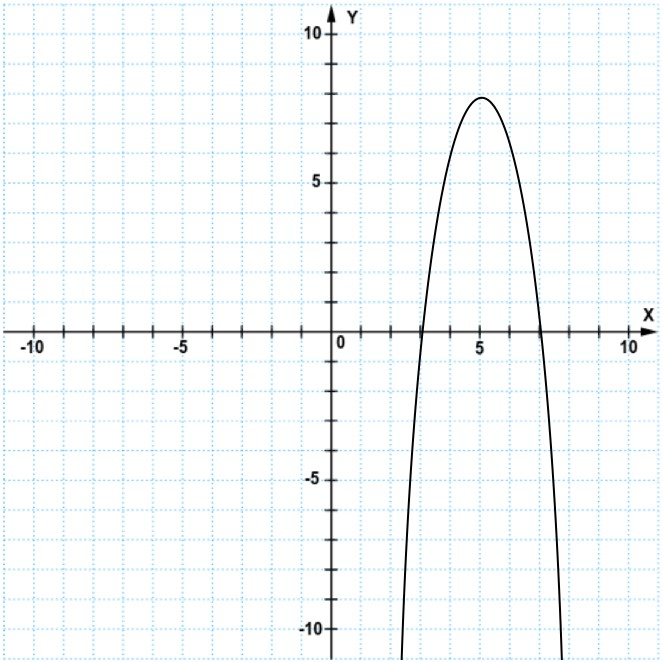
\includegraphics[scale=0.7]{pm1.jpeg}
		\end{figure}

		\begin{mdframed}[%
			linecolor=white,%
			innertopmargin=\topskip,
			shadowsize=0,%
			innertopmargin=5,%
			innerbottommargin=5,%
			leftmargin=10,%
			rightmargin=10,%
			backgroundcolor=gray!20,%
			innertopmargin=0pt,]
			\vspace{0.2cm}
			\textbf{\textit{Zadanie 1.11.1 (0-1)}}
			
			
		\end{mdframed}
	
		Zapisz poniżej w postaci przedziału zbiór wartości powyższej funkcji kwadratowej. \vspace{1cm}
		
		....................................................................................................................................
		
		\begin{mdframed}[%
			linecolor=white,%
			innertopmargin=\topskip,
			shadowsize=0,%
			innertopmargin=5,%
			innerbottommargin=5,%
			leftmargin=10,%
			rightmargin=10,%
			backgroundcolor=gray!20,%
			innertopmargin=0pt,]
			\vspace{0.2cm}
			\textbf{\textit{Zadanie 1.11.2 (0-3)}}
			\\
			Wyznacz wzór funkcji kwadratowej w postaci ogólnej.
		\end{mdframed}
	
		\newpage
		\begin{mdframed}[%
			linecolor=white,%
			innertopmargin=\topskip,
			shadowsize=0,%
			innertopmargin=5,%
			innerbottommargin=5,%
			leftmargin=10,%
			rightmargin=10,%
			backgroundcolor=gray!20,%
			innertopmargin=0pt,]
			\vspace{0.2cm}
			\textbf{\textit{Zadanie 1.11.3 (0-1)}}\\
			\textbf{Dokończ zdanie. Wybierz właściwą odpowiedź spośród podanych.}
			
		\end{mdframed}
	
	Funkcję $g(x)-f(x-2)-2$ przedstawiono na wykresie
	
		\begin{figure}[h]
			\centering
			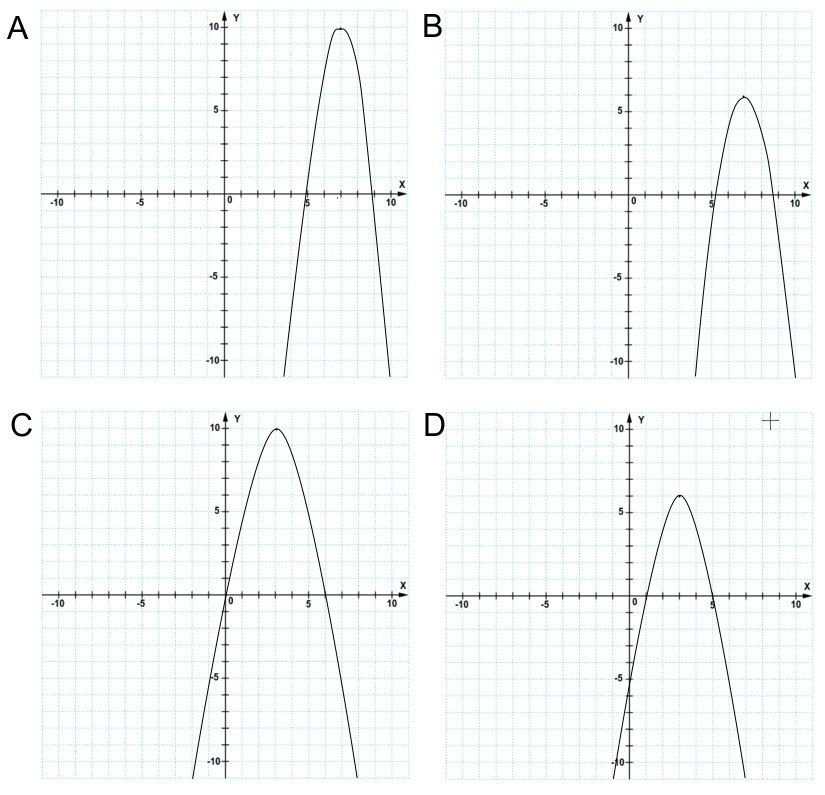
\includegraphics[scale=0.5]{pm2.jpeg}
		\end{figure}
	
	%%%%%%%%%%%%%%%%%%%%%%%%%%%%%
	
	\begin{zad}[0-1]
		\textbf{Dokończ zdanie. Wybierz właściwą odpowiedź spośród podanych.}
	\end{zad} 
	
	W labolatorium badno próbki pewnego kamienia pozaziemskiego. Naukowcy są w stanie ustalić wiek powstania danego kamienia na postawie śladu węgla wewnątrz danej probówki za pomocą uproszczonej formuły $T(x)= 1000\cdot2^{-x \cdot 10^{-10}}$ w jednej uncji próbki (wyrażonej w mg), gdzie x to jest czas życia danej probówki.
	\\\\
	Przy badaniu tej próbki otrzymano, że w jednej uncji znajduje się 62,5g węgla. Zatem ten kamień ma
	
	\vspace{0.5cm}
	\begin{tabular}{p{3.5cm} p{3.5cm} p{3.5cm} p{3.5cm}}
		\textbf{A. }$4\cdot10^{10}$ lat&
		\textbf{B. }$4000$ lat&
		\textbf{C. }$62,5\cdot10^{10}$ lat&
		\textbf{D. }$62,5\cdot 10^{10000} $ lat\\
	\end{tabular}
	\newpage
	
	%%%%%%%%%%%%%%%%%%%%%%%%%%%%%
	
	\begin{zad}[0-1]
		\textbf{Oceń prawdziwość poniższych stwierdzeń. Wybierz P, jeśli stwierdzenie jest prawdziwe, albo F – jeśli jest fałszywe.}
	\end{zad} 
	
	Dany jest ciąg rekurencyjny określony wzorem
	
	$$\left\{\begin{array}{l}
		a_{n+1}=a_n\cdot2n\\
		a_n=3
	\end{array}\right.$$
	
	\vspace{0.5cm}
	\begin{tabular}{|p{12.5cm}|p{1cm}|p{1cm}|}

		\hline
		\begin{flushleft}
			Ciąg $a_n$ jest ciągiem geometrycznym.
		\end{flushleft}&\begin{center}
			\textbf{P}
		\end{center}&\begin{center}
		\textbf{F}
	\end{center}\\
		\hline
		\begin{flushleft}
			Ciąg $a_n$ jest ciągiem monotonicznym.
		\end{flushleft}&\begin{center}
			\textbf{P}
		\end{center}&\begin{center}
			\textbf{F}
		\end{center}\\
		\hline
	\end{tabular}

	%%%%%%%%%%%%%%%%%%%%%%%%%%%%%
	
	\begin{zad}[0-1]
		\textbf{Oceń prawdziwość poniższych stwierdzeń. Wybierz P, jeśli stwierdzenie jest prawdziwe, albo F – jeśli jest fałszywe.}
	\end{zad} 

	Suma pierwszego i dwunastego wyrazu pewnego ciągu arytmetycznego wynosi 4, natomiast różnica piątego i siódmego wyrazu tego ciągu wynosi 4.
	
	\vspace{0.5cm}
	\begin{tabular}{|p{12.5cm}|p{1cm}|p{1cm}|}
		
		\hline
		\begin{flushleft}
			Ciąg ten jest rosnący.
		\end{flushleft}&\begin{center}
			\textbf{P}
		\end{center}&\begin{center}
			\textbf{F}
		\end{center}\\
		\hline
		\begin{flushleft}
			Pierwszy wyraz tego ciągu wynosi 13.
		\end{flushleft}&\begin{center}
			\textbf{P}
		\end{center}&\begin{center}
			\textbf{F}
		\end{center}\\
		\hline
	\end{tabular}
	
	\begin{zad}[0-4]
		Dany jest pewien trzywyrazowy ciąg arytmetyczny $(x,y,z)$. Średnia arytmetyczna tego ciągu to 7. Jeżeli drugi wyraz tego ciągu zmniejszylibyśmy o 1, to otrzymalibyśmy ciąg geometryczny. Wyznacz wyrazy tego ciągu.
	\end{zad} 

	%%%%%%%%%%%%%%%%%%%%%%%%%%%%%
	
	\begin{zad}[0-1]
		\textbf{Dokończ zdanie. Wybierz właściwą odpowiedź spośród podanych.}
	\end{zad} 
	
	Dla pewnego ostrego kąta $\alpha$ dane jest, że $\sin\alpha = \frac{2\sqrt{2}}{3}$. Wówczas $\text{tg }\alpha$ wynosi
	
	\vspace{0.5cm}
	\begin{tabular}{p{3.5cm} p{3.5cm} p{3.5cm} p{3.5cm}}
		\textbf{A. }$2\sqrt{2}$&
		\textbf{B. }$\frac{\sqrt{2}}{4}$&
		\textbf{C. }$3$&
		\textbf{D. }$\frac{1}{3}$\\
	\end{tabular}

	\newpage
	
	%%%%%%%%%%%%%%%%%%%%%%%%%%%%%
	
	\begin{zad}[0-1]
		\textbf{Dokończ zdanie. Wybierz właściwą odpowiedź spośród podanych.}
	\end{zad} 
	
	Dany jest trójkąt równoramienny o ramieniu długości 20 i kącie między ramionami $150^\circ$. Wówczas pole tego trójkąta jest równe
	
	\vspace{0.5cm}
	\begin{tabular}{p{3.5cm} p{3.5cm} p{3.5cm} p{3.5cm}}
		\textbf{A. }$200\sqrt{3}$&
		\textbf{B. }$200$&
		\textbf{C. }$100\sqrt{3}$&
		\textbf{D. }$100$\\
	\end{tabular}

	\begin{zad}[0-1]
		\textbf{Dokończ zdanie. Wybierz właściwą odpowiedź spośród podanych.}
	\end{zad} 
	
	Dane są dwa okręgi
	$$o_1\;:\;(x-2)^2+(y-k)^2=81$$
	$$o_2\;:\;(x+2)^2+(y-6)^2=16$$
	
	Okręgi te są styczne wewnętrznie kiedy $k$ jest równe
	
	\vspace{0.5cm}
	\begin{tabular}{p{3.5cm} p{3.5cm} p{3.5cm} p{3.5cm}}
		\textbf{A. }$3-3\sqrt{15}$&
		\textbf{B. }$3$&
		\textbf{C. }$6$&
		\textbf{D. }$-1$\\
	\end{tabular}
	
	
	

\end{document}